\chapter{Aufgabenstellung}
\section{Motivation}
In der medizinischen Forschung werden h�ufig Tierversuche durchgef�hrt, die am h�ufigst verwendete Tierart sind M�use und Ratten.
Die M�use und Ratten werden in K�figen gehalten, um R�ckschl�sse auf den medizinische Zustand zu erhalten wird die K�rpertemperatur gemessen. Um diesen Zeitaufwand einzusparen soll die Messung und Auswertung der Temperatur automatisiert werden. F�r diesen Zweck wurde ein Prototyp mit einer Infrarot-Kamera zur Tierbeobachtung erstellt. 
Ziel dieser Belegarbeit ist es, ein thermisches Modell zu erstellen, welches die infrarot Aufnahme einer Maus in mehreren Pixel darstellt.

\section{Beleg - Spezifikation}
Es wird f�r die erstellten Modelle eine statisch thermische Simulation durchgef�hrt. Eine Optimierung hinsichtlich der geometrischen Anordnung, sowie ein Vergleich der bisherigen Ergebnisse in Bezug auf gegenseitige Beeinflussung, zeitliche Erw�rmung und Abk�hlung. Daraufhin ist mit dem besten Ergebnis eine Simulation durchzuf�hren die den zeitlichen Verlauf von Verschiebungseffekten sichtbar macht. 
\begin{table}[bh]
	\centering
	\caption{Beleg - Spezifikation}
	\begin{tabular}{l p{9cm} } 
			\rowcolor[gray]{.8}	 Leiterplatte (LP):& 50x50 mm, 7x7 Bauelemente, 2 Lagig (Toplayer Bauelemente, Bottomlayer Leiterbahnen)\\
			Anordung& in der Mitte der LP 3x3 Pixel mit gleicher Verlustleistung (au�er das mittlere Element) 	  					\\	
			\rowcolor[gray]{.8}Ausf�hrung: & jeweils mit Transistoren SMD (SOT23) und SMD Widerst�nden (1206)\\
			Verlustleistungen:& 50 mW, 100 mW, 150 mW 
		%Feld&\multicolumn{2}{c}{}\\
	\end{tabular}
	\label{tab:beleg_anforderungen}
\end{table}

%\newpage
\begin{center}
	\begin{minipage}[!ht]{.8\textwidth}
			\captionsetup{type=figure}
			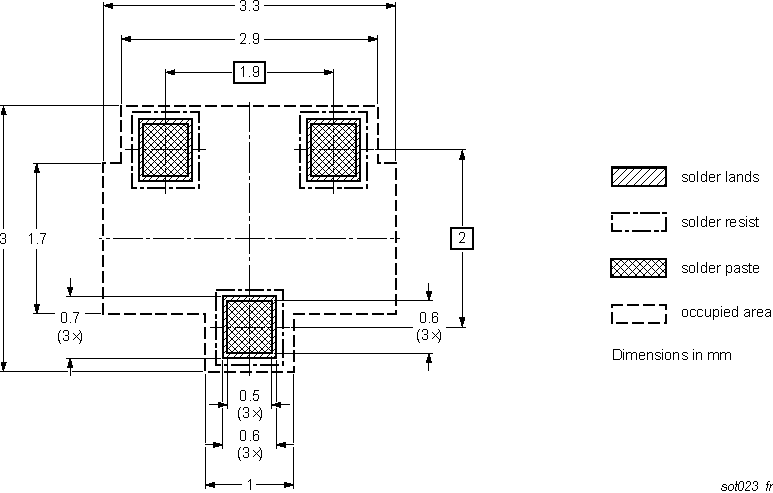
\includegraphics[width=1\linewidth]{bilder/sot23footprint.pdf}
			\caption{Transistor- Dimensionen als SOT23 Geh�uses, \\Quelle: NXP - PDTC114E Datenblatt S.10 }
			\label{fig:Messaufbau}
	\end{minipage}
	\hspace{1cm}
	\begin{minipage}[!ht]{0.45\textwidth}
		\centering 
		\captionsetup{type=figure}
		%\def\svgwidth{200pt}
		%\includegraphics[width=1\linewidth]{bilder/grafik_messaufbau.pdf}
		%	\includegraphics{bilder/messstand_biegebalken}
		%\resizebox{1.02\textwidth}{!}{\input{bilder/grafik_messaufbau.pdf_tex}}
		\caption{Informationsverlauf des Messaufbaus}
		\label{graf:Invormationsverlauf_Messaufbau}
	\end{minipage}
\end{center}

		
\newpage


\section{Antrieb}
Zur Kraft�bertragung wird eine Kombination aus einem Schrittmotor und einem Linearantrieb verwendet. In Tabelle \ref{tab:Motoreigenschaften} sind die Eigenschaften der vorhandenen Schrittmotoren gegen�bergestellt. Der Schrittmotor f�r die vertikale Richtung besitzt einen maximalen Phasenstrom von $4,2 \text{ A}_\text{eff}$ und ein maximales Moment von $1,7 \text{ Nm}$. Der Motor f�r die horizontale Richtung ist kleiner, besitzt ein geringeres Drehmoment von $0,59 \text{ Nm}$ und einen Phasenstrom von $0,6 \text{ A}$.



%Die Spindel f�r die vertikale Achse hat eine Steigung von $4 \text{ mm}$, die f�r die horizontale Achse besitzt $2 \text{ mm}$ Steigung (siehe Tabelle \ref{tab:Spindeleigenschaften}).

\section{Kommunikation}
Die Kraftregelung (Bild \ref{graf:Invormationsverlauf_Messaufbau}) besteht aus drei Teilbereichen: der \gls{dms}-Messschaltung, dem Kraftregler und der Motorsteuerung. Die Messschaltung und die Kraftregelung wird unter anderem mit Atmel Mikrocontrollern durchgef�hrt. Um einen Datenaustausch zwischen den Controllern gew�hrleisten zu k�nnen, wird eine Kommunikation �ber einen \gls{i2c} Datenbus festgelegt.

